\section{Data Processing}

Before concluding anything from the data, they are first analysed to check if the assumptions made are valid. The assumptions include a stationary channel, uncorrelated samples and finally that the data is Rayleigh distributed.

\subsection{Raw data}

In total 4,184,460 samples have been collected, the values are represented in \autoref{fig:rawFadingMeas}. All the space samples has been concatenated to visualize the data.

\begin{figure}[H]
\centering
\includegraphics[height = \textwidth, angle = -90]{figures/rawFadingMeas.pdf}
\caption{The measured samples separated in frequency and space.}
\label{fig:rawFadingMeas}
\end{figure}


\subsection{Stationarity}\label{sec:meas_stationarity}
The stationarity of channel is verified by checking if the measurements conform to the criteria of \gls{WSSUS}. This is done by checking \gls{WSS} in the temporal domain and \gls{US} in the spatial domain. The criteria for this is a constant mean and a autocorrelation that is only dependent on delay between samples \citep[ch. 5]{The_Mobile_Radio_Propagation_Channelbook}. 

\textbf{Temporal domain mean}

The data is structured in 3 domains (frequency, antenna, walk/space), with N, M and K being the number of points in each dimension. To analyse stationarity in frequency an average is taken across the other two domains:

\begin{equation}\label{eq:freqMean}
\overrightarrow{freqData}_{(n)} = \frac{1}{K\cdot M}\sum_{k = 1}^{K}\sum_{m = 1}^{M} \textbf{data}_{(n,m,k)}
\end{equation}
\begin{where}
\va{$\overrightarrow{freqData}$}{is the mean value for the different frequencies}{1}
\va{$K$}{is the number of elements in the antenna dimension, 3}{1}
\va{$M$}{is the number of spatial points measured, 34020}{1}
\va{$\textbf{data}$}{is the measured data as ratio of input to output}{1}
\end{where}


\begin{figure}[H]
\centering
%\includegraphics[height = \textwidth, angle = -90]{figures/meanFading.pdf}
% This file was created by matlab2tikz.
%
%The latest updates can be retrieved from
%  http://www.mathworks.com/matlabcentral/fileexchange/22022-matlab2tikz-matlab2tikz
%where you can also make suggestions and rate matlab2tikz.
%
\definecolor{mycolor1}{rgb}{0.00000,0.44700,0.74100}%
%
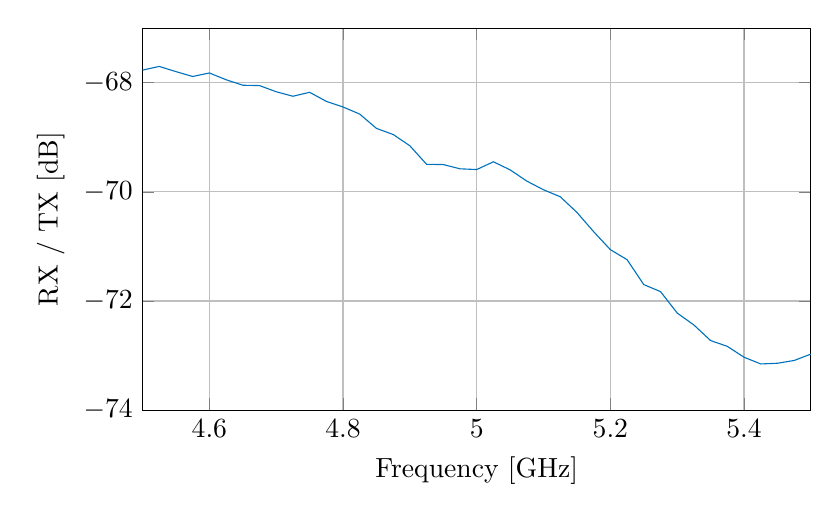
\begin{tikzpicture}

\begin{axis}[%
width=0.7\textwidth,
height=0.4\textwidth,
at={(0.758in,0.481in)},
scale only axis,
xmin=4.5,
xmax=5.5,
xlabel={Frequency [GHz]},
xmajorgrids,
ymin=-74,
ymax=-67,
ylabel={RX / TX [dB]},
ymajorgrids,
axis background/.style={fill=white}
]
\addplot [color=mycolor1,solid,forget plot]
  table[row sep=crcr]{%
4.5	-67.7676892980713\\
4.525	-67.7004021954752\\
4.55	-67.7955301958539\\
4.575	-67.8845412993962\\
4.6	-67.8205218880063\\
4.625	-67.9439627079413\\
4.65	-68.04512612016\\
4.675	-68.051565781706\\
4.7	-68.1644910960917\\
4.725	-68.2469599638715\\
4.75	-68.1744447064323\\
4.775	-68.3408515759533\\
4.8	-68.4431912057773\\
4.825	-68.5744291919179\\
4.85	-68.8363636692087\\
4.875	-68.9480881021396\\
4.9	-69.1549059751271\\
4.925	-69.4947511904151\\
4.95	-69.4993310363175\\
4.975	-69.5769572316811\\
5	-69.5906628312393\\
5.025	-69.4483437709345\\
5.05	-69.5961078771687\\
5.075	-69.8026690275714\\
5.1	-69.9616513128938\\
5.125	-70.0889574328478\\
5.15	-70.3770813009446\\
5.175	-70.7298661505624\\
5.2	-71.0591359058608\\
5.225	-71.2429090613138\\
5.25	-71.6994261918864\\
5.275	-71.8280447931612\\
5.3	-72.2209086728416\\
5.325	-72.4401711956896\\
5.35	-72.7258613771483\\
5.375	-72.8313187431047\\
5.4	-73.0312002594864\\
5.425	-73.154105653938\\
5.45	-73.1413033949649\\
5.475	-73.0904973481192\\
5.5	-72.9729692416908\\
};
\end{axis}
\end{tikzpicture}%
\caption{Average values across the frequency as per \autoref{eq:freqMean}, with values converted from linear to dB.}
\label{fig:meanFading}
\end{figure}

A drop of around 5 dB across the frequency can be seen from \autoref{fig:meanFading}, this drop can be linked to two factors: first the antenna gain varies with around 2 dB across the frequency span known from \appref{ant_adix}, secondly from the free space path loss model it can be seen that there is a drop of 1.75 dB going from 4.5 GHz to 5.5 GHz. The data will be adjusted by these factors:

\begin{equation}
\textbf{data2}_{(:,:,k)} =  \textbf{data}_{(:,:,k)} \oslash \left(\overrightarrow{freqData}\cdot \overrightarrow{ones(1,M)}\right), \quad k = (1,2,...,K)
\end{equation}
\begin{where}
\va{$\textbf{data2}$}{is the data normalized with regards to frequency imbalance}{1}
\va{$\overrightarrow{ones(1,M)}$}{is a vector of ones with dimension 1xM}{1}
\end{where}

\textbf{Spatial domain mean}

Similar to temporal domain the average is taken across the other domains, it is assumed that the antenna domain is stationary due to small area occupied by the antennas. The average is found based on the frequency corrected data as:

\begin{equation}\label{eq:spaceMean}
\overrightarrow{spaceData}_{(k)} = \frac{1}{N\cdot M}\sum_{n = 1}^{N}\sum_{m = 1}^{M} \textbf{data2}_{(n,m,k)}
\end{equation}
\begin{where}
\va{$\overrightarrow{spaceData}$}{is the mean value for the different spatial samples}{1}
\va{$N$}{is the number of frequency points measured}{1}
\end{where}


To visualize the data it is restructured such that it matches the area from \autoref{meas_area}. The data was collected by walking back and forth in the room with approximately 42 sweeps per meter or 210 sweeps per stretch. As every second stretch was walking back it has to be reversed to visualize the samples side by side. 



\begin{figure}[H]
\captionsetup{belowskip=0em}
\centering
\begin{subfigure}[b]{0.29\textwidth}
\includegraphics[width=\textwidth]{figures/Not_Norm_space_1.png}
\caption{Low height \\ approx. 70 cm}
\label{Not_norm_low}
\end{subfigure}
\begin{subfigure}[b]{0.29\textwidth}
\includegraphics[width=\textwidth]{figures/Not_Norm_space_2.png}
\caption{Medium height \\ approx. 120 cm}
\label{Not_norm_medium}
\end{subfigure}
\begin{subfigure}[b]{0.29\textwidth}
\includegraphics[width=\textwidth]{figures/Not_Norm_space_3.png}
\caption{High height \\ approx. 170 cm}
\label{Not_norm_high}
\end{subfigure}
\begin{subfigure}[b]{0.1\textwidth}
\includegraphics[width=\textwidth]{figures/Not_Norm_space_colorbar.png}
\end{subfigure}
\captionsetup{belowskip=-1.5em}
\caption{The measurements are restructured to be approximately where they were measured compared to each other.}
\label{fig:Not_norm_space}
\end{figure}

It can be seen from \autoref{fig:Not_norm_space} that the power level in the middle of the room is stronger than on the borders. The reason for this is believed to be the directionality of the TX antenna. The TX antenna was located outside and pointing into the room as can be seen on \autoref{antennadoor}, so the main lobe might have been reflected from the wall directly to the middle of the measurement area. Because of this the area can not be said to be stationary, to combat this a moving average is used to normalize the mean power level across the area. The drawback of using a moving average is that it might affect the fading in the measurement. As many point as possible should therefore be averaged over the minimize the influence on fading, however if the average is taken over too many points the stationarity issue would not be solved. It is chosen to average across 41 spatial samples.

\begin{align}
&\overrightarrow{MA} = \frac{1}{41}\cdot \Big(\overrightarrow{spaceData}*\overrightarrow{ones(1,41)}\Big) \\
\textbf{data3}_{(:,:,k)} = \textbf{data2}_{(:,:,k)} &\oslash \left(\overrightarrow{MA}_{\left(\frac{41-1}{2}:N+\frac{41-1}{2}\right)}\cdot \overrightarrow{ones(1,M)}\right), \quad k = (1,2,...,K)
\end{align}
\begin{where}
\va{$\overrightarrow{MA}$}{is the moving average of the spatial samples}{1}
\va{$\textbf{data3}$}{is the normalized data in frequency and space}{1}
\end{where}

The result of the normalization can be seen on \autoref{fig:Norm_space}.

\begin{figure}[H]
\captionsetup{belowskip=0em}
\centering
\begin{subfigure}[b]{0.29\textwidth}
\includegraphics[width=\textwidth]{figures/Norm_space_1.png}
\caption{Low height \\ approx. 70 cm}
\label{Norm_low}
\end{subfigure}
\begin{subfigure}[b]{0.29\textwidth}
\includegraphics[width=\textwidth]{figures/Norm_space_2.png}
\caption{Medium height \\ approx. 120 cm}
\label{Norm_medium}
\end{subfigure}
\begin{subfigure}[b]{0.29\textwidth}
\includegraphics[width=\textwidth]{figures/Norm_space_3.png}
\caption{High height \\ approx. 170 cm}
\label{Norm_high}
\end{subfigure}
\begin{subfigure}[b]{0.1\textwidth}
\includegraphics[width=\textwidth]{figures/Norm_space_colorbar.png}
\end{subfigure}
\captionsetup{belowskip=-1.5em}
\caption{The normalize measurements is restructured to be approximately where they was measured compared to each other.}
\label{fig:Norm_space}
\end{figure}

It can be concluded the mean was not constant during the measurement, however due to the normalization the spatial mean of \textit{data3} can be considered to be constant across all measurements. The last check to see if the channel is \gls{WSSUS} is to verify that the autocovariance function is only dependent on sample shift. This is also done in both the temporal and spatial domain.

\textbf{Temporal domain correlation}

It needs to be checked if:
\begin{equation}\label{eq:autocovariance_check}
R_f(n,n+\Delta n) = R_f(\Delta n) 
\end{equation}
\begin{where}
\va{$R_f$}{is the autocorrelation of the frequency samples}{1}
\va{$\Delta n$}{is the sample shift in frequency}{1}
\end{where}

First the sample mean and sample variance is found for each point in space as:

\begin{align}
\mathbf{\mu}_{f,(m,k)} &= \frac{1}{N}\sum_{n = 1}^{N} \textbf{data3}_{(n,m,k)} \\
\textbf{s}_{f,(m,k)}^2 &= \frac{1}{N-1}\sum_{n = 1}^{N} \left( \textbf{data3}_{(n,m,k)} - \mathbf{\mu}_{f,(m,k)} \right)^2 
\end{align}
\begin{where}
\va{$\mu_{f}$}{is the sample mean of the frequency samples}{1}
\va{$\textbf{s}^2_f$}{is the sample variance of the frequency samples}{1}
\end{where}

For each element in space the cross covariance matrix is found as the sample covariance divided with the sample variance:
\begin{equation}
C_f(n,n+\Delta n,m,k) = \frac{\left(\textbf{data3}_{(n,m,k)}-\mu_{f,(m,k)}\right)\cdot \left(\textbf{data3}_{(n+\Delta n,m,k)}-\mu_{f,(m,k)}\right)}{\textbf{s}_{f,(m,k)}^2}
\end{equation}
\begin{where}
\va{$C_f$}{is the cross correlation between sample ($n,m,k$) and ($n+\Delta n,m,k$)}{1}
\end{where}

The average across all space samples are then found as:
\begin{equation}
R_f(n,n+\Delta n) = \frac{1}{K\cdot M}\sum_{k = 1}^{K}\sum_{m = 1}^{M} C_f(n,n+\Delta n,m,k)
\end{equation}


The final step is to show that \autoref{eq:autocovariance_check} is true. If this is true all diagonal lines in R would have a constant value, that implies that the variance across the diagonal line elements is 0. 

\begin{align}
&\mu_{R_f}(\Delta n) = \frac{1}{N-|\Delta n|}\sum_{n = 1}^{N-|\Delta n|} R_f(n,n+\Delta n) \label{EQcor}\\
s_{R_f}^2(\Delta n) = &\frac{1}{N-|\Delta n|-1}\sum_{n = 1}^{N-|\Delta n|} \left( R_f(n,n+\Delta n) - \mu_{R_f}(\Delta n) \right)^2 \label{eq:variance_of_covariance}
\end{align}
\begin{where}
\va{$\mu_{R_f}$}{is the mean autocorrelation function}{1}
\va{$s_{R_f}^2$}{is the variance of the autocorrelation samples}{1}
\end{where}

The result of \autoref{eq:variance_of_covariance} can be seen in \autoref{fig:var_freq}, as $R_f(n,n+\Delta n)$ is an even function only the positive values of $\Delta n$ is shown.

\begin{figure}[H]
\centering
% This file was created by matlab2tikz.
%
%The latest updates can be retrieved from
%  http://www.mathworks.com/matlabcentral/fileexchange/22022-matlab2tikz-matlab2tikz
%where you can also make suggestions and rate matlab2tikz.
%
\definecolor{mycolor1}{rgb}{0.00000,0.44700,0.74100}%
%
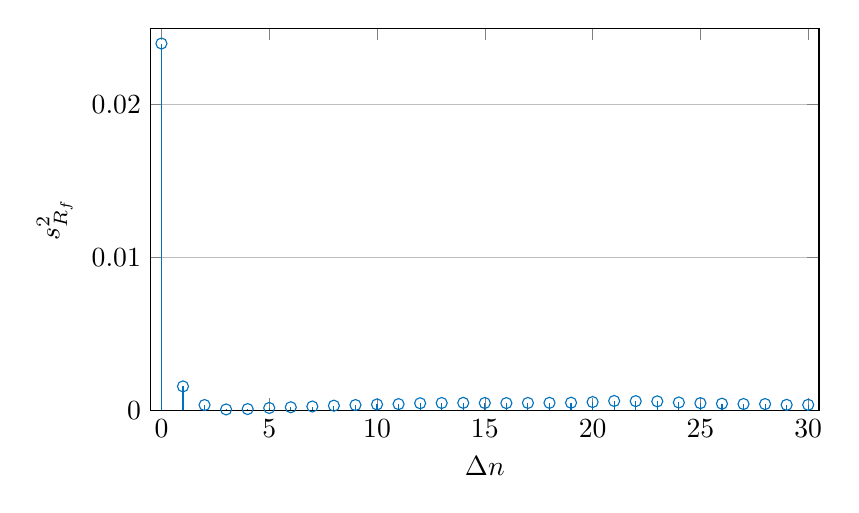
\begin{tikzpicture}

\begin{axis}[%
width=0.7\textwidth,
height=0.4\textwidth,
at={(0.758in,0.481in)},
scale only axis,
scaled y ticks = false,
y tick label style={/pgf/number format/fixed, /pgf/number format/precision=4},
xmin=-0.5,
xmax=30.5,
xlabel = $\Delta n$,
ymajorgrids,
ymin=0,
ymax=0.025,
ylabel = $s_{R_f}^2$,
axis background/.style={fill=white}
]
\addplot[ycomb,color=mycolor1,solid,mark=o,mark options={solid},forget plot] plot table[row sep=crcr] {%
0	0.0239994535570242\\
1	0.00155347561399147\\
2	0.000333132530399424\\
3	4.42952964310783e-05\\
4	6.91463617776512e-05\\
5	0.000140552123495002\\
6	0.00018743076774746\\
7	0.000236684877793891\\
8	0.000291324870818997\\
9	0.000331910825749033\\
10	0.000371904245897478\\
11	0.00039280175885968\\
12	0.000448157932287774\\
13	0.00046607349315818\\
14	0.000475171842259718\\
15	0.000466606546009396\\
16	0.000459354658352822\\
17	0.000469730606803343\\
18	0.000476346246957716\\
19	0.000483291253215299\\
20	0.00052789844826084\\
21	0.000599881231205234\\
22	0.000587411820871848\\
23	0.000573953897934685\\
24	0.000499460691984749\\
25	0.000456959069830855\\
26	0.000421847342166333\\
27	0.000400310575870904\\
28	0.000396373029801933\\
29	0.000345580578532402\\
30	0.000347170193328993\\
};
\end{axis}
\end{tikzpicture}%
\caption{Variance of autocorrelation with respect to $\Delta n$.}
\label{fig:var_freq}
\end{figure}

\autoref{fig:var_freq} shows that all the variences are quite low, this is a very good indicator that the autocorrelation is only dependent on $\Delta n$ and therefore the data is WSS.

\textbf{Spatial domain correlation}

Analogously to the temporal domain the process is repeated for the spatial domain. The result of which can be seen on \autoref{fig:var_space}.

\begin{figure}[H]
\centering
% This file was created by matlab2tikz.
%
%The latest updates can be retrieved from
%  http://www.mathworks.com/matlabcentral/fileexchange/22022-matlab2tikz-matlab2tikz
%where you can also make suggestions and rate matlab2tikz.
%
\definecolor{mycolor1}{rgb}{0.00000,0.44700,0.74100}%
%
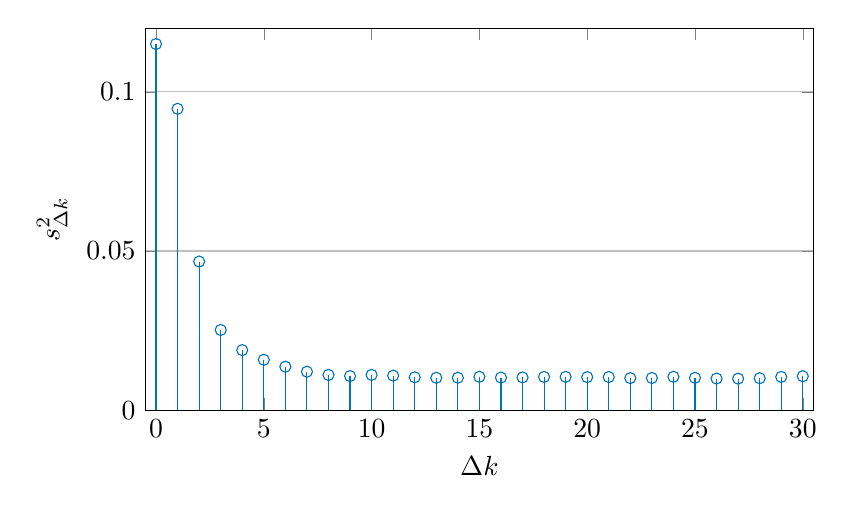
\begin{tikzpicture}

\begin{axis}[%
width=0.7\textwidth,
height=0.4\textwidth,
at={(0.758in,0.481in)},
scale only axis,
y tick label style={/pgf/number format/fixed},
xlabel = $\Delta k$,
xmin=-0.5,
xmax=30.5,
ymajorgrids,
ymin=0,
ymax=0.12,
ylabel = $s^2_{\Delta k}$,
axis background/.style={fill=white}
]
\addplot[ycomb,color=mycolor1,solid,mark=o,mark options={solid},forget plot] plot table[row sep=crcr] {%
0	0.115045606834225\\
1	0.0946784511696748\\
2	0.0466923552353349\\
3	0.0251857163185419\\
4	0.0188648457284451\\
5	0.0158108437878889\\
6	0.0136428154850336\\
7	0.0120691680816066\\
8	0.0110553269974913\\
9	0.0107016887908107\\
10	0.0110733653475015\\
11	0.0108419533225932\\
12	0.0103199849300731\\
13	0.0101549456533492\\
14	0.0101751416039882\\
15	0.010467137052642\\
16	0.0102326076635985\\
17	0.0102798250233889\\
18	0.0104377402107261\\
19	0.0104501815917102\\
20	0.010370718973987\\
21	0.0103919293729459\\
22	0.0100594042395687\\
23	0.0100951562316132\\
24	0.01047263290787\\
25	0.0101459206592842\\
26	0.00991026231424316\\
27	0.00989028804544289\\
28	0.0100207717725258\\
29	0.0104324957762442\\
30	0.0106517054365681\\
};
\end{axis}
\end{tikzpicture}%
\caption{Variance of autocorrelation with respect to $\Delta k$.}
\label{fig:var_space}
\end{figure}

\autoref{fig:var_space} gives a clear indication that the variance is not nearly as small as for the frequency domain, this could be connected to the problem discovered from \autoref{fig:Not_norm_space}. These two problems indicates that a dominant component has been received from the direction of the TX antenna. It is however assumed that the effect of this component is only big enough to be seen in the stationarity analysis and not in the result of the fading characteristic.
